\section{Hardware}
Při vytváření stanice bylo nejprve potřeba zvolit vhodný micropočítač pro připojení měřicích komponentů. Nakonec jsme vybrali platformu Arduino,
konkrétně model ESP8266WiFi, který nám umožnil, nejen zapojit všechny různé komponenty potřebné pro měření, ale i připojení k interneru.

\subsection{Propojení se serverem}
Po zapnutí se stanice připojí k internetu zapomocí Wifi a zaregistruje na backendu (popsáno v kapitole \ref{komunikace}). Jakmile stanice dostane od serveru odpověd s 
JSON Web Tokenem, uloží si ho a při každém opeslání dat na server ho použije k prokázání totožnosti.

\subsection{Měření teploty a vlhkosti}
Pro měření teploty a vlhkosti byl použit Digitální teploměr Adafruit AM2320 Sensor\cite{teplomer}. V případě nebylo zapotřebí vymýšlet jak cokoli měřit,
protože senzor je připojen přes I2C interface, ze kterého program pouze čte již změřené hodnoty.
\begin{figure}[h] 
    \centering
    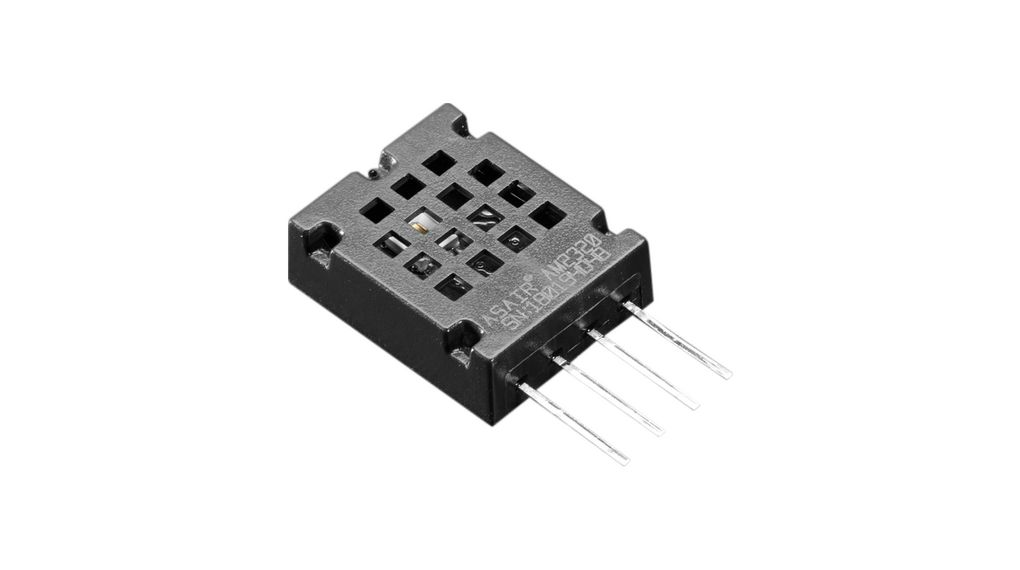
\includegraphics[width=0.25\textwidth]{images/Adafruit-AM2320.jpg}
    \caption{Teploměr a vlhkoměr}
\end{figure}

\subsection{Měření tlaku}
Měření tlaku je zhruba stejně přímočaré jako měření teploty, což znamená, že se o měření stará sensor\cite{tlakoměr},
který zapojen přes I2C interface, ze kterého program čte hodnotu klaku v jednotce Pa.

\begin{figure}[h] 
    \centering
    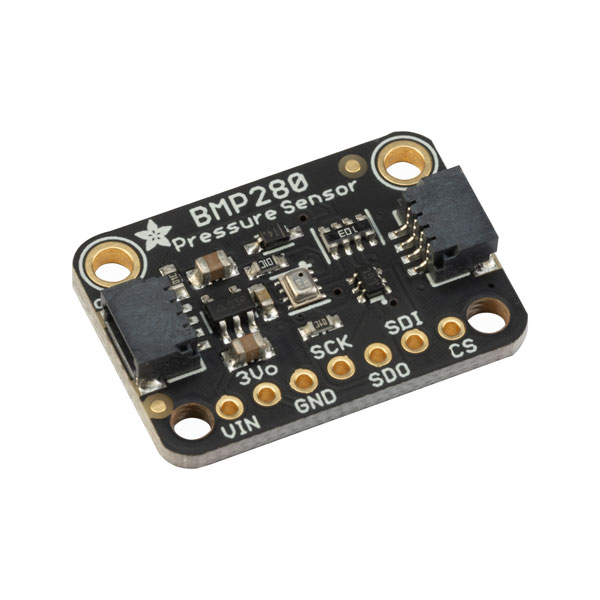
\includegraphics[width=0.25\textwidth]{images/Adafruit-BMP280.jpg}
    \caption{Tlakoměr}
\end{figure}
\subsection{Měření větru}

\subsection{Měření deště}

\subsection{Prostor pro zlepšení}
